% Options for packages loaded elsewhere
\PassOptionsToPackage{unicode}{hyperref}
\PassOptionsToPackage{hyphens}{url}
\PassOptionsToPackage{dvipsnames,svgnames,x11names}{xcolor}
%
\documentclass[
  letterpaper,
  DIV=11,
  numbers=noendperiod]{scrreport}

\usepackage{amsmath,amssymb}
\usepackage{lmodern}
\usepackage{iftex}
\ifPDFTeX
  \usepackage[T1]{fontenc}
  \usepackage[utf8]{inputenc}
  \usepackage{textcomp} % provide euro and other symbols
\else % if luatex or xetex
  \usepackage{unicode-math}
  \defaultfontfeatures{Scale=MatchLowercase}
  \defaultfontfeatures[\rmfamily]{Ligatures=TeX,Scale=1}
\fi
% Use upquote if available, for straight quotes in verbatim environments
\IfFileExists{upquote.sty}{\usepackage{upquote}}{}
\IfFileExists{microtype.sty}{% use microtype if available
  \usepackage[]{microtype}
  \UseMicrotypeSet[protrusion]{basicmath} % disable protrusion for tt fonts
}{}
\makeatletter
\@ifundefined{KOMAClassName}{% if non-KOMA class
  \IfFileExists{parskip.sty}{%
    \usepackage{parskip}
  }{% else
    \setlength{\parindent}{0pt}
    \setlength{\parskip}{6pt plus 2pt minus 1pt}}
}{% if KOMA class
  \KOMAoptions{parskip=half}}
\makeatother
\usepackage{xcolor}
\setlength{\emergencystretch}{3em} % prevent overfull lines
\setcounter{secnumdepth}{5}
% Make \paragraph and \subparagraph free-standing
\ifx\paragraph\undefined\else
  \let\oldparagraph\paragraph
  \renewcommand{\paragraph}[1]{\oldparagraph{#1}\mbox{}}
\fi
\ifx\subparagraph\undefined\else
  \let\oldsubparagraph\subparagraph
  \renewcommand{\subparagraph}[1]{\oldsubparagraph{#1}\mbox{}}
\fi

\usepackage{color}
\usepackage{fancyvrb}
\newcommand{\VerbBar}{|}
\newcommand{\VERB}{\Verb[commandchars=\\\{\}]}
\DefineVerbatimEnvironment{Highlighting}{Verbatim}{commandchars=\\\{\}}
% Add ',fontsize=\small' for more characters per line
\usepackage{framed}
\definecolor{shadecolor}{RGB}{241,243,245}
\newenvironment{Shaded}{\begin{snugshade}}{\end{snugshade}}
\newcommand{\AlertTok}[1]{\textcolor[rgb]{0.68,0.00,0.00}{#1}}
\newcommand{\AnnotationTok}[1]{\textcolor[rgb]{0.37,0.37,0.37}{#1}}
\newcommand{\AttributeTok}[1]{\textcolor[rgb]{0.40,0.45,0.13}{#1}}
\newcommand{\BaseNTok}[1]{\textcolor[rgb]{0.68,0.00,0.00}{#1}}
\newcommand{\BuiltInTok}[1]{\textcolor[rgb]{0.00,0.23,0.31}{#1}}
\newcommand{\CharTok}[1]{\textcolor[rgb]{0.13,0.47,0.30}{#1}}
\newcommand{\CommentTok}[1]{\textcolor[rgb]{0.37,0.37,0.37}{#1}}
\newcommand{\CommentVarTok}[1]{\textcolor[rgb]{0.37,0.37,0.37}{\textit{#1}}}
\newcommand{\ConstantTok}[1]{\textcolor[rgb]{0.56,0.35,0.01}{#1}}
\newcommand{\ControlFlowTok}[1]{\textcolor[rgb]{0.00,0.23,0.31}{#1}}
\newcommand{\DataTypeTok}[1]{\textcolor[rgb]{0.68,0.00,0.00}{#1}}
\newcommand{\DecValTok}[1]{\textcolor[rgb]{0.68,0.00,0.00}{#1}}
\newcommand{\DocumentationTok}[1]{\textcolor[rgb]{0.37,0.37,0.37}{\textit{#1}}}
\newcommand{\ErrorTok}[1]{\textcolor[rgb]{0.68,0.00,0.00}{#1}}
\newcommand{\ExtensionTok}[1]{\textcolor[rgb]{0.00,0.23,0.31}{#1}}
\newcommand{\FloatTok}[1]{\textcolor[rgb]{0.68,0.00,0.00}{#1}}
\newcommand{\FunctionTok}[1]{\textcolor[rgb]{0.28,0.35,0.67}{#1}}
\newcommand{\ImportTok}[1]{\textcolor[rgb]{0.00,0.46,0.62}{#1}}
\newcommand{\InformationTok}[1]{\textcolor[rgb]{0.37,0.37,0.37}{#1}}
\newcommand{\KeywordTok}[1]{\textcolor[rgb]{0.00,0.23,0.31}{#1}}
\newcommand{\NormalTok}[1]{\textcolor[rgb]{0.00,0.23,0.31}{#1}}
\newcommand{\OperatorTok}[1]{\textcolor[rgb]{0.37,0.37,0.37}{#1}}
\newcommand{\OtherTok}[1]{\textcolor[rgb]{0.00,0.23,0.31}{#1}}
\newcommand{\PreprocessorTok}[1]{\textcolor[rgb]{0.68,0.00,0.00}{#1}}
\newcommand{\RegionMarkerTok}[1]{\textcolor[rgb]{0.00,0.23,0.31}{#1}}
\newcommand{\SpecialCharTok}[1]{\textcolor[rgb]{0.37,0.37,0.37}{#1}}
\newcommand{\SpecialStringTok}[1]{\textcolor[rgb]{0.13,0.47,0.30}{#1}}
\newcommand{\StringTok}[1]{\textcolor[rgb]{0.13,0.47,0.30}{#1}}
\newcommand{\VariableTok}[1]{\textcolor[rgb]{0.07,0.07,0.07}{#1}}
\newcommand{\VerbatimStringTok}[1]{\textcolor[rgb]{0.13,0.47,0.30}{#1}}
\newcommand{\WarningTok}[1]{\textcolor[rgb]{0.37,0.37,0.37}{\textit{#1}}}

\providecommand{\tightlist}{%
  \setlength{\itemsep}{0pt}\setlength{\parskip}{0pt}}\usepackage{longtable,booktabs,array}
\usepackage{calc} % for calculating minipage widths
% Correct order of tables after \paragraph or \subparagraph
\usepackage{etoolbox}
\makeatletter
\patchcmd\longtable{\par}{\if@noskipsec\mbox{}\fi\par}{}{}
\makeatother
% Allow footnotes in longtable head/foot
\IfFileExists{footnotehyper.sty}{\usepackage{footnotehyper}}{\usepackage{footnote}}
\makesavenoteenv{longtable}
\usepackage{graphicx}
\makeatletter
\def\maxwidth{\ifdim\Gin@nat@width>\linewidth\linewidth\else\Gin@nat@width\fi}
\def\maxheight{\ifdim\Gin@nat@height>\textheight\textheight\else\Gin@nat@height\fi}
\makeatother
% Scale images if necessary, so that they will not overflow the page
% margins by default, and it is still possible to overwrite the defaults
% using explicit options in \includegraphics[width, height, ...]{}
\setkeys{Gin}{width=\maxwidth,height=\maxheight,keepaspectratio}
% Set default figure placement to htbp
\makeatletter
\def\fps@figure{htbp}
\makeatother

\KOMAoption{captions}{tableheading}
\makeatletter
\makeatother
\makeatletter
\@ifpackageloaded{bookmark}{}{\usepackage{bookmark}}
\makeatother
\makeatletter
\@ifpackageloaded{caption}{}{\usepackage{caption}}
\AtBeginDocument{%
\ifdefined\contentsname
  \renewcommand*\contentsname{Table of contents}
\else
  \newcommand\contentsname{Table of contents}
\fi
\ifdefined\listfigurename
  \renewcommand*\listfigurename{List of Figures}
\else
  \newcommand\listfigurename{List of Figures}
\fi
\ifdefined\listtablename
  \renewcommand*\listtablename{List of Tables}
\else
  \newcommand\listtablename{List of Tables}
\fi
\ifdefined\figurename
  \renewcommand*\figurename{Figure}
\else
  \newcommand\figurename{Figure}
\fi
\ifdefined\tablename
  \renewcommand*\tablename{Table}
\else
  \newcommand\tablename{Table}
\fi
}
\@ifpackageloaded{float}{}{\usepackage{float}}
\floatstyle{ruled}
\@ifundefined{c@chapter}{\newfloat{codelisting}{h}{lop}}{\newfloat{codelisting}{h}{lop}[chapter]}
\floatname{codelisting}{Listing}
\newcommand*\listoflistings{\listof{codelisting}{List of Listings}}
\makeatother
\makeatletter
\@ifpackageloaded{caption}{}{\usepackage{caption}}
\@ifpackageloaded{subcaption}{}{\usepackage{subcaption}}
\makeatother
\makeatletter
\@ifpackageloaded{tcolorbox}{}{\usepackage[many]{tcolorbox}}
\makeatother
\makeatletter
\@ifundefined{shadecolor}{\definecolor{shadecolor}{rgb}{.97, .97, .97}}
\makeatother
\makeatletter
\makeatother
\ifLuaTeX
  \usepackage{selnolig}  % disable illegal ligatures
\fi
\IfFileExists{bookmark.sty}{\usepackage{bookmark}}{\usepackage{hyperref}}
\IfFileExists{xurl.sty}{\usepackage{xurl}}{} % add URL line breaks if available
\urlstyle{same} % disable monospaced font for URLs
\hypersetup{
  pdftitle={Testing quarto book},
  pdfauthor={Luis R. Gonzalez},
  colorlinks=true,
  linkcolor={blue},
  filecolor={Maroon},
  citecolor={Blue},
  urlcolor={Blue},
  pdfcreator={LaTeX via pandoc}}

\title{Testing quarto book}
\author{Luis R. Gonzalez}
\date{8/18/2022}

\begin{document}
\maketitle
\ifdefined\Shaded\renewenvironment{Shaded}{\begin{tcolorbox}[boxrule=0pt, sharp corners, frame hidden, breakable, interior hidden, borderline west={3pt}{0pt}{shadecolor}, enhanced]}{\end{tcolorbox}}\fi

\renewcommand*\contentsname{Table of contents}
{
\hypersetup{linkcolor=}
\setcounter{tocdepth}{2}
\tableofcontents
}
\bookmarksetup{startatroot}

\hypertarget{test}{%
\chapter{test}\label{test}}

This is a Quarto website.

To learn more about Quarto websites visit
\url{https://quarto.org/docs/websites}.

\bookmarksetup{startatroot}

\hypertarget{testing-cross-reference-with-holoviews-charts}{%
\chapter{Testing cross-reference with holoviews
charts}\label{testing-cross-reference-with-holoviews-charts}}

Luis R. Gonzalez\\
Aug 20, 2022

\hfill\break

::: \{.cell 0=`h' 1=`i' 2=`d' 3=`e' execution\_count=1\}

\begin{Shaded}
\begin{Highlighting}[]
\ImportTok{import}\NormalTok{ pandas }\ImportTok{as}\NormalTok{ pd}
\ImportTok{from}\NormalTok{ sklearn.datasets }\ImportTok{import}\NormalTok{ load\_iris}
\ImportTok{from}\NormalTok{ pandas }\ImportTok{import}\NormalTok{ util}
\ImportTok{import}\NormalTok{ seaborn }\ImportTok{as}\NormalTok{ sns}
\end{Highlighting}
\end{Shaded}

:::

::: \{.cell 0=`h' 1=`i' 2=`d' 3=`e' execution\_count=2\}

\begin{Shaded}
\begin{Highlighting}[]
\NormalTok{pd.options.plotting.backend }\OperatorTok{=} \StringTok{"holoviews"}
\end{Highlighting}
\end{Shaded}

:::

::: \{.cell 0=`h' 1=`i' 2=`d' 3=`e' execution\_count=3\}

\begin{Shaded}
\begin{Highlighting}[]
\NormalTok{data }\OperatorTok{=}\NormalTok{ load\_iris()}
\end{Highlighting}
\end{Shaded}

:::

::: \{.cell 0=`h' 1=`i' 2=`d' 3=`e' execution\_count=4\}

\begin{Shaded}
\begin{Highlighting}[]
\NormalTok{df }\OperatorTok{=}\NormalTok{ util.testing.makeTimeDataFrame()}
\end{Highlighting}
\end{Shaded}

\begin{verbatim}
/home/gonluisr/miniconda3/envs/conda_dev/lib/python3.9/site-packages/pandas/util/__init__.py:15: FutureWarning: pandas.util.testing is deprecated. Use the functions in the public API at pandas.testing instead.
  import pandas.util.testing
\end{verbatim}

:::

::: \{.cell 0=`h' 1=`i' 2=`d' 3=`e' execution\_count=5\}

\begin{Shaded}
\begin{Highlighting}[]
\NormalTok{df.head()}
\end{Highlighting}
\end{Shaded}

\begin{longtable}[]{@{}lllll@{}}
\toprule()
& A & B & C & D \\
\midrule()
\endhead
2000-01-03 & -0.582207 & -1.000480 & 0.323955 & 0.007650 \\
2000-01-04 & 0.424007 & 0.775093 & -0.127669 & -0.930395 \\
2000-01-05 & 0.411417 & -0.783818 & -0.345699 & -0.415395 \\
2000-01-06 & 0.251328 & 0.623833 & -0.278011 & -0.412769 \\
2000-01-07 & 0.357047 & 0.098218 & 2.741289 & 0.199595 \\
\bottomrule()
\end{longtable}

:::

::: \{.cell 0=`h' 1=`i' 2=`d' 3=`e' execution\_count=6\}

\begin{Shaded}
\begin{Highlighting}[]
\NormalTok{df.reset\_index().rename(columns}\OperatorTok{=}\NormalTok{\{}\StringTok{\textquotesingle{}index\textquotesingle{}}\NormalTok{:}\StringTok{\textquotesingle{}Date\textquotesingle{}}\NormalTok{\}).groupby([pd.Grouper(key}\OperatorTok{=}\StringTok{\textquotesingle{}Date\textquotesingle{}}\NormalTok{,freq}\OperatorTok{=}\StringTok{\textquotesingle{}w{-}MON\textquotesingle{}}\NormalTok{)]).}\BuiltInTok{sum}\NormalTok{()}
\end{Highlighting}
\end{Shaded}

\begin{longtable}[]{@{}lllll@{}}
\toprule()
& A & B & C & D \\
Date & & & & \\
\midrule()
\endhead
2000-01-03 & -0.582207 & -1.000480 & 0.323955 & 0.007650 \\
2000-01-10 & -0.234743 & 2.167578 & 2.652053 & -1.093058 \\
2000-01-17 & 0.013742 & -2.757776 & 2.834797 & 3.770157 \\
2000-01-24 & 1.523045 & -1.485811 & -1.243673 & -0.963989 \\
2000-01-31 & -1.848256 & 0.759201 & -0.621093 & -0.670768 \\
2000-02-07 & -1.006205 & 0.135843 & -2.535127 & -3.419145 \\
2000-02-14 & -4.913442 & -0.683123 & -0.694445 & 0.557568 \\
\bottomrule()
\end{longtable}

:::

::: \{.cell 0=`h' 1=`i' 2=`d' 3=`e' execution\_count=7\}

\begin{Shaded}
\begin{Highlighting}[]
\NormalTok{df }\OperatorTok{=}\NormalTok{ df.assign(max\_value }\OperatorTok{=}\NormalTok{ df.}\BuiltInTok{max}\NormalTok{(axis}\OperatorTok{=}\DecValTok{1}\NormalTok{))}
\end{Highlighting}
\end{Shaded}

:::

::: \{.cell 0=`h' 1=`i' 2=`d' 3=`e' execution\_count=8\}

\begin{Shaded}
\begin{Highlighting}[]
\KeywordTok{def}\NormalTok{ classify(df):}
    \ControlFlowTok{if}\NormalTok{ df[}\StringTok{\textquotesingle{}max\_value\textquotesingle{}}\NormalTok{] }\OperatorTok{\textgreater{}=} \DecValTok{1}\NormalTok{:}
        \ControlFlowTok{return} \StringTok{\textquotesingle{}High\textquotesingle{}}
    \ControlFlowTok{if}\NormalTok{ df[}\StringTok{\textquotesingle{}max\_value\textquotesingle{}}\NormalTok{] }\OperatorTok{\textgreater{}} \FloatTok{0.5} \KeywordTok{and}\NormalTok{ df[}\StringTok{\textquotesingle{}max\_value\textquotesingle{}}\NormalTok{] }\OperatorTok{\textless{}} \DecValTok{1}\NormalTok{:}
        \ControlFlowTok{return} \StringTok{\textquotesingle{}Medium\textquotesingle{}}
    \ControlFlowTok{if}\NormalTok{ df[}\StringTok{\textquotesingle{}max\_value\textquotesingle{}}\NormalTok{] }\OperatorTok{\textless{}} \FloatTok{0.5}\NormalTok{:}
        \ControlFlowTok{return} \StringTok{\textquotesingle{}Low\textquotesingle{}}
\end{Highlighting}
\end{Shaded}

:::

::: \{.cell 0=`h' 1=`i' 2=`d' 3=`e' execution\_count=9\}

\begin{Shaded}
\begin{Highlighting}[]
\NormalTok{df }\OperatorTok{=}\NormalTok{ df.assign(Category }\OperatorTok{=}\NormalTok{ df.}\BuiltInTok{apply}\NormalTok{(classify,axis}\OperatorTok{=}\DecValTok{1}\NormalTok{))}
\end{Highlighting}
\end{Shaded}

:::

::: \{.cell 0=`h' 1=`i' 2=`d' 3=`e' execution\_count=10\}

\begin{Shaded}
\begin{Highlighting}[]
\NormalTok{df[}\StringTok{\textquotesingle{}Category\textquotesingle{}}\NormalTok{] }\OperatorTok{=}\NormalTok{ df[}\StringTok{\textquotesingle{}Category\textquotesingle{}}\NormalTok{].astype(}\StringTok{"category"}\NormalTok{)}
\end{Highlighting}
\end{Shaded}

:::

::: \{.cell 0=`h' 1=`i' 2=`d' 3=`e' execution\_count=11\}

\begin{Shaded}
\begin{Highlighting}[]
\NormalTok{df}
\end{Highlighting}
\end{Shaded}

\begin{longtable}[]{@{}lllllll@{}}
\toprule()
& A & B & C & D & max\_value & Category \\
\midrule()
\endhead
2000-01-03 & -0.582207 & -1.000480 & 0.323955 & 0.007650 & 0.323955 &
Low \\
2000-01-04 & 0.424007 & 0.775093 & -0.127669 & -0.930395 & 0.775093 &
Medium \\
2000-01-05 & 0.411417 & -0.783818 & -0.345699 & -0.415395 & 0.411417 &
Low \\
2000-01-06 & 0.251328 & 0.623833 & -0.278011 & -0.412769 & 0.623833 &
Medium \\
2000-01-07 & 0.357047 & 0.098218 & 2.741289 & 0.199595 & 2.741289 &
High \\
2000-01-10 & -1.678541 & 1.454251 & 0.662143 & 0.465905 & 1.454251 &
High \\
2000-01-11 & 0.966773 & 0.322669 & 1.030897 & 0.297324 & 1.030897 &
High \\
2000-01-12 & 0.640741 & 0.021307 & 0.941115 & 0.848067 & 0.941115 &
Medium \\
2000-01-13 & -0.366762 & -0.951611 & 1.395349 & 1.230894 & 1.395349 &
High \\
2000-01-14 & -0.857458 & -1.627424 & -1.701975 & 1.309590 & 1.309590 &
High \\
2000-01-17 & -0.369552 & -0.522716 & 1.169411 & 0.084282 & 1.169411 &
High \\
2000-01-18 & 0.183638 & 0.736659 & -0.305887 & 0.388168 & 0.736659 &
Medium \\
2000-01-19 & 0.366433 & -1.072837 & -1.111730 & -0.427861 & 0.366433 &
Low \\
2000-01-20 & 0.585825 & 0.347986 & -0.934388 & 0.410635 & 0.585825 &
Medium \\
2000-01-21 & 0.728517 & -0.715842 & 1.069210 & -0.164306 & 1.069210 &
High \\
2000-01-24 & -0.341368 & -0.781776 & 0.039122 & -1.170624 & 0.039122 &
Low \\
2000-01-25 & -0.926737 & 0.399972 & 0.507149 & 2.065153 & 2.065153 &
High \\
2000-01-26 & 0.203486 & 0.653138 & -1.691324 & 0.776340 & 0.776340 &
Medium \\
2000-01-27 & 0.311465 & -0.332699 & 0.237594 & -1.473875 & 0.311465 &
Low \\
2000-01-28 & -0.826008 & -1.235476 & 0.331498 & -0.972064 & 0.331498 &
Low \\
2000-01-31 & -0.610462 & 1.274265 & -0.006010 & -1.066323 & 1.274265 &
High \\
2000-02-01 & 1.705305 & -0.255701 & -0.466338 & -2.782992 & 1.705305 &
High \\
2000-02-02 & -0.531286 & 0.220349 & -0.882575 & -1.492108 & 0.220349 &
Low \\
2000-02-03 & 0.011553 & 0.053408 & -0.556360 & 0.512802 & 0.512802 &
Medium \\
2000-02-04 & -1.645071 & -1.363826 & -0.339289 & 0.479332 & 0.479332 &
Low \\
2000-02-07 & -0.546705 & 1.481613 & -0.290566 & -0.136178 & 1.481613 &
High \\
2000-02-08 & -1.319182 & -0.473713 & -0.714132 & 0.218225 & 0.218225 &
Low \\
2000-02-09 & 0.121003 & 1.047676 & 0.142332 & 0.822883 & 1.047676 &
High \\
2000-02-10 & -1.286180 & -0.918822 & -0.301173 & 0.150331 & 0.150331 &
Low \\
2000-02-11 & -2.429082 & -0.338264 & 0.178528 & -0.633871 & 0.178528 &
Low \\
\bottomrule()
\end{longtable}

:::

See Figure~\ref{fig-plot}

\begin{figure}

{\centering 

\begin{figure}

{\centering 

\begin{verbatim}
Unable to display output for mime type(s): application/javascript, application/vnd.holoviews_load.v0+json
\end{verbatim}

}

\caption{Holoviews example}

\end{figure}

\begin{figure}

{\centering 

\begin{verbatim}
Unable to display output for mime type(s): application/javascript, application/vnd.holoviews_load.v0+json
\end{verbatim}

}

\caption{\textbf{?(caption)}}

\end{figure}

\begin{figure}

{\centering 

\begin{verbatim}
Unable to display output for mime type(s): text/html
\end{verbatim}

}

\caption{\textbf{?(caption)}}

\end{figure}

\begin{figure}

{\centering 

\begin{verbatim}
Unable to display output for mime type(s): 
\end{verbatim}

}

\caption{\textbf{?(caption)}}

\end{figure}

\begin{figure}

{\centering 

\begin{verbatim}
:NdLayout   [Variable]
   :Curve   [index]   (value)
\end{verbatim}

}

\caption{\textbf{?(caption)}}

\end{figure}

}

\caption{\label{fig-plot}\textbf{?(caption)}}

\end{figure}

\begin{figure}

{\centering \includegraphics{./testing_files/figure-pdf/fig-pairplot-output-1.png}

}

\caption{\label{fig-pairplot}Seaborn pairplot example}

\end{figure}

\bookmarksetup{startatroot}

\hypertarget{testing-cross-reference-with-holoviews-charts-1}{%
\chapter{Testing cross-reference with holoviews
charts}\label{testing-cross-reference-with-holoviews-charts-1}}

Luis R. Gonzalez\\
Aug 20, 2022

\hfill\break

::: \{.cell 0=`h' 1=`i' 2=`d' 3=`e' execution\_count=2\}

\begin{Shaded}
\begin{Highlighting}[]
\ImportTok{import}\NormalTok{ pandas }\ImportTok{as}\NormalTok{ pd}
\ImportTok{from}\NormalTok{ sklearn.datasets }\ImportTok{import}\NormalTok{ load\_iris}
\ImportTok{from}\NormalTok{ pandas }\ImportTok{import}\NormalTok{ util}
\ImportTok{import}\NormalTok{ seaborn }\ImportTok{as}\NormalTok{ sns}
\end{Highlighting}
\end{Shaded}

:::

::: \{.cell 0=`h' 1=`i' 2=`d' 3=`e' execution\_count=3\}

\begin{Shaded}
\begin{Highlighting}[]
\NormalTok{pd.options.plotting.backend }\OperatorTok{=} \StringTok{"holoviews"}
\end{Highlighting}
\end{Shaded}

:::

::: \{.cell 0=`h' 1=`i' 2=`d' 3=`e' execution\_count=4\}

\begin{Shaded}
\begin{Highlighting}[]
\NormalTok{data }\OperatorTok{=}\NormalTok{ load\_iris()}
\end{Highlighting}
\end{Shaded}

:::

::: \{.cell 0=`h' 1=`i' 2=`d' 3=`e' execution\_count=5\}

\begin{Shaded}
\begin{Highlighting}[]
\NormalTok{df }\OperatorTok{=}\NormalTok{ util.testing.makeTimeDataFrame()}
\end{Highlighting}
\end{Shaded}

\begin{verbatim}
/home/gonluisr/miniconda3/envs/conda_dev/lib/python3.9/site-packages/pandas/util/__init__.py:15: FutureWarning: pandas.util.testing is deprecated. Use the functions in the public API at pandas.testing instead.
  import pandas.util.testing
\end{verbatim}

:::

::: \{.cell 0=`h' 1=`i' 2=`d' 3=`e' execution\_count=6\}

\begin{Shaded}
\begin{Highlighting}[]
\NormalTok{df.head()}
\end{Highlighting}
\end{Shaded}

\begin{longtable}[]{@{}lllll@{}}
\toprule()
& A & B & C & D \\
\midrule()
\endhead
2000-01-03 & 1.126988 & -1.147395 & 0.187442 & -0.630229 \\
2000-01-04 & 1.201789 & -0.000927 & 0.723552 & -0.852234 \\
2000-01-05 & -0.468707 & 0.151884 & -0.785213 & 0.847470 \\
2000-01-06 & 1.116639 & 0.803649 & 1.077325 & -1.361432 \\
2000-01-07 & 0.155205 & -1.248513 & 0.752966 & -0.201408 \\
\bottomrule()
\end{longtable}

:::

::: \{.cell 0=`h' 1=`i' 2=`d' 3=`e' execution\_count=7\}

\begin{Shaded}
\begin{Highlighting}[]
\NormalTok{df.reset\_index().rename(columns}\OperatorTok{=}\NormalTok{\{}\StringTok{\textquotesingle{}index\textquotesingle{}}\NormalTok{:}\StringTok{\textquotesingle{}Date\textquotesingle{}}\NormalTok{\}).groupby([pd.Grouper(key}\OperatorTok{=}\StringTok{\textquotesingle{}Date\textquotesingle{}}\NormalTok{,freq}\OperatorTok{=}\StringTok{\textquotesingle{}M\textquotesingle{}}\NormalTok{)]).}\BuiltInTok{sum}\NormalTok{()}
\end{Highlighting}
\end{Shaded}

\begin{longtable}[]{@{}lllll@{}}
\toprule()
& A & B & C & D \\
Date & & & & \\
\midrule()
\endhead
2000-01-31 & 5.767612 & -0.264180 & 5.102825 & 0.220061 \\
2000-02-29 & 1.149543 & -2.713967 & 1.188419 & 1.265752 \\
\bottomrule()
\end{longtable}

:::

::: \{.cell 0=`h' 1=`i' 2=`d' 3=`e' execution\_count=8\}

\begin{Shaded}
\begin{Highlighting}[]
\NormalTok{df }\OperatorTok{=}\NormalTok{ df.assign(max\_value }\OperatorTok{=}\NormalTok{ df.}\BuiltInTok{max}\NormalTok{(axis}\OperatorTok{=}\DecValTok{1}\NormalTok{))}
\end{Highlighting}
\end{Shaded}

:::

::: \{.cell 0=`h' 1=`i' 2=`d' 3=`e' execution\_count=9\}

\begin{Shaded}
\begin{Highlighting}[]
\KeywordTok{def}\NormalTok{ classify(df):}
    \ControlFlowTok{if}\NormalTok{ df[}\StringTok{\textquotesingle{}max\_value\textquotesingle{}}\NormalTok{] }\OperatorTok{\textgreater{}=} \DecValTok{1}\NormalTok{:}
        \ControlFlowTok{return} \StringTok{\textquotesingle{}High\textquotesingle{}}
    \ControlFlowTok{if}\NormalTok{ df[}\StringTok{\textquotesingle{}max\_value\textquotesingle{}}\NormalTok{] }\OperatorTok{\textgreater{}} \FloatTok{0.5} \KeywordTok{and}\NormalTok{ df[}\StringTok{\textquotesingle{}max\_value\textquotesingle{}}\NormalTok{] }\OperatorTok{\textless{}} \DecValTok{1}\NormalTok{:}
        \ControlFlowTok{return} \StringTok{\textquotesingle{}Medium\textquotesingle{}}
    \ControlFlowTok{if}\NormalTok{ df[}\StringTok{\textquotesingle{}max\_value\textquotesingle{}}\NormalTok{] }\OperatorTok{\textless{}} \FloatTok{0.5}\NormalTok{:}
        \ControlFlowTok{return} \StringTok{\textquotesingle{}Low\textquotesingle{}}
\end{Highlighting}
\end{Shaded}

:::

::: \{.cell 0=`h' 1=`i' 2=`d' 3=`e' execution\_count=10\}

\begin{Shaded}
\begin{Highlighting}[]
\NormalTok{df }\OperatorTok{=}\NormalTok{ df.assign(Category }\OperatorTok{=}\NormalTok{ df.}\BuiltInTok{apply}\NormalTok{(classify,axis}\OperatorTok{=}\DecValTok{1}\NormalTok{))}
\end{Highlighting}
\end{Shaded}

:::

::: \{.cell 0=`h' 1=`i' 2=`d' 3=`e' execution\_count=11\}

\begin{Shaded}
\begin{Highlighting}[]
\NormalTok{df[}\StringTok{\textquotesingle{}Category\textquotesingle{}}\NormalTok{] }\OperatorTok{=}\NormalTok{ df[}\StringTok{\textquotesingle{}Category\textquotesingle{}}\NormalTok{].astype(}\StringTok{"category"}\NormalTok{)}
\end{Highlighting}
\end{Shaded}

:::

::: \{.cell 0=`h' 1=`i' 2=`d' 3=`e' execution\_count=12\}

\begin{Shaded}
\begin{Highlighting}[]
\NormalTok{df}
\end{Highlighting}
\end{Shaded}

\begin{longtable}[]{@{}lllllll@{}}
\toprule()
& A & B & C & D & max\_value & Category \\
\midrule()
\endhead
2000-01-03 & 1.126988 & -1.147395 & 0.187442 & -0.630229 & 1.126988 &
High \\
2000-01-04 & 1.201789 & -0.000927 & 0.723552 & -0.852234 & 1.201789 &
High \\
2000-01-05 & -0.468707 & 0.151884 & -0.785213 & 0.847470 & 0.847470 &
Medium \\
2000-01-06 & 1.116639 & 0.803649 & 1.077325 & -1.361432 & 1.116639 &
High \\
2000-01-07 & 0.155205 & -1.248513 & 0.752966 & -0.201408 & 0.752966 &
Medium \\
2000-01-10 & -1.106183 & -1.103509 & 0.734816 & -1.539371 & 0.734816 &
Medium \\
2000-01-11 & 0.749808 & 0.457427 & 0.236783 & 0.007655 & 0.749808 &
Medium \\
2000-01-12 & 1.345924 & -0.701440 & 0.402120 & 1.055362 & 1.345924 &
High \\
2000-01-13 & -1.630626 & -1.373218 & 1.154692 & 0.145866 & 1.154692 &
High \\
2000-01-14 & 0.985955 & -0.233816 & -0.108853 & 2.763228 & 2.763228 &
High \\
2000-01-17 & 0.149018 & -0.906383 & 2.091126 & -1.161566 & 2.091126 &
High \\
2000-01-18 & -0.025945 & -0.186756 & 0.399277 & 0.506350 & 0.506350 &
Medium \\
2000-01-19 & 1.649071 & -0.814364 & 0.397560 & 0.633919 & 1.649071 &
High \\
2000-01-20 & -0.231581 & 0.796854 & 0.050179 & -0.109894 & 0.796854 &
Medium \\
2000-01-21 & 0.839475 & -0.337561 & -1.344820 & -0.391172 & 0.839475 &
Medium \\
2000-01-24 & -0.023087 & 0.814299 & -0.134823 & 0.585606 & 0.814299 &
Medium \\
2000-01-25 & 1.085229 & 0.636130 & -0.585263 & -1.639097 & 1.085229 &
High \\
2000-01-26 & -0.771849 & 0.366846 & 1.133055 & 1.377471 & 1.377471 &
High \\
2000-01-27 & -0.304234 & 0.866607 & -0.785338 & 0.050379 & 0.866607 &
Medium \\
2000-01-28 & 0.053750 & 2.026548 & -1.510660 & -0.497465 & 2.026548 &
High \\
2000-01-31 & -0.129026 & 0.869457 & 1.016903 & 0.630623 & 1.016903 &
High \\
2000-02-01 & -1.085380 & -0.030132 & 1.435229 & -1.153119 & 1.435229 &
High \\
2000-02-02 & 1.549394 & -0.795620 & 2.160895 & 0.318606 & 2.160895 &
High \\
2000-02-03 & -0.344825 & 0.094948 & -0.529953 & 0.037532 & 0.094948 &
Low \\
2000-02-04 & 0.061480 & -0.018256 & 1.055836 & 0.739908 & 1.055836 &
High \\
2000-02-07 & 0.923516 & 0.428145 & -1.522212 & 2.815199 & 2.815199 &
High \\
2000-02-08 & -0.963635 & -1.178148 & -0.603736 & 0.370689 & 0.370689 &
Low \\
2000-02-09 & -0.151846 & -1.137036 & -1.355825 & 0.382550 & 0.382550 &
Low \\
2000-02-10 & -0.445424 & -0.114888 & 0.003508 & -1.178604 & 0.003508 &
Low \\
2000-02-11 & 1.606264 & 0.037020 & 0.544675 & -1.067008 & 1.606264 &
High \\
\bottomrule()
\end{longtable}

:::

See Figure~\ref{fig-plot} and Figure~\ref{fig-plot-copy}

\begin{figure}

{\centering 

\begin{figure}

{\centering 

\begin{verbatim}
Unable to display output for mime type(s): application/javascript, application/vnd.holoviews_load.v0+json
\end{verbatim}

}

\caption{Holoviews example}

\end{figure}

\begin{figure}

{\centering 

\begin{verbatim}
Unable to display output for mime type(s): application/javascript, application/vnd.holoviews_load.v0+json
\end{verbatim}

}

\caption{\textbf{?(caption)}}

\end{figure}

\begin{figure}

{\centering 

\begin{verbatim}
Unable to display output for mime type(s): text/html
\end{verbatim}

}

\caption{\textbf{?(caption)}}

\end{figure}

\begin{figure}

{\centering 

\begin{verbatim}
Unable to display output for mime type(s): 
\end{verbatim}

}

\caption{\textbf{?(caption)}}

\end{figure}

\begin{figure}

{\centering 

\begin{verbatim}
:NdOverlay   [Variable]
   :Curve   [index]   (value)
\end{verbatim}

}

\caption{\textbf{?(caption)}}

\end{figure}

}

\caption{\label{fig-plot-copy}\textbf{?(caption)}}

\end{figure}

\begin{figure}

{\centering \includegraphics{./testing_copy_files/figure-pdf/fig-pairplot-output-1.png}

}

\caption{\label{fig-pairplot}Seaborn pairplot example}

\end{figure}

\bookmarksetup{startatroot}

\hypertarget{about}{%
\chapter{About}\label{about}}

About this site



\end{document}
